%%%%%%%%%%%%%%%%%%%%%%%%%%%%%%%%%%%%%%%%%
% Simple Sectioned Essay Template
% LaTeX Template
%
% This template has been downloaded from:
% http://www.latextemplates.com
%
% Note:
% The \lipsum[#] commands throughout this template generate dummy text
% to fill the template out. These commands should all be removed when 
% writing essay content.
%
%%%%%%%%%%%%%%%%%%%%%%%%%%%%%%%%%%%%%%%%%

%----------------------------------------------------------------------------------------
%	PACKAGES AND OTHER DOCUMENT CONFIGURATIONS
%----------------------------------------------------------------------------------------

\documentclass[12pt]{article} % Default font size is 12pt, it can be changed here

\usepackage{geometry} % Required to change the page size to A4
\geometry{a4paper} % Set the page size to be A4 as opposed to the default US Letter
\usepackage[utf8]{inputenc}

\usepackage{graphicx} % Required for including pictures

\usepackage{float} % Allows putting an [H] in \begin{figure} to specify the exact location of the figure
\usepackage{wrapfig} % Allows in-line images such as the example fish picture

\usepackage{lipsum} % Used for inserting dummy 'Lorem ipsum' text into the template
\usepackage{color}

\linespread{1.2} % Line spacing

%\setlength\parindent{0pt} % Uncomment to remove all indentation from paragraphs

\graphicspath{{Figures/}} % Specifies the directory where pictures are stored

\usepackage[hidelinks]{hyperref}
\usepackage{tabularx}

\begin{document}

%----------------------------------------------------------------------------------------
%	TITLE PAGE
%----------------------------------------------------------------------------------------

\begin{titlepage}

\newcommand{\HRule}{\rule{\linewidth}{0.5mm}} % Defines a new command for the horizontal lines, change thickness here

\center % Center everything on the page

\textsc{\LARGE Hochschule Mannheim}\\[1.5cm] % Name of your university/college
\textsc{\Large Algorithmen für moderne Rechnerarchitekturen}\\[0.5cm] % Major heading such as course name
\textsc{\large  }\\[0.5cm] % Minor heading such as course title

\HRule \\[0.4cm]
{ \huge \bfseries Methoden zur Börsenkursvorhersage}\\[0.4cm] % Title of your document
\HRule \\[1.5cm]

{\centering \emph{Autoren:}}
\\

\begin{minipage}{0.4\textwidth}
\begin{flushleft} \large
Marc \textsc{Misoch} 
\end{flushleft}
\end{minipage}
~
\begin{minipage}{0.4\textwidth}
\begin{flushright} \large
David \textsc{Marquant} % Supervisor's Name
\end{flushright}
\end{minipage}\\[4cm]

{\large \today}\\[3cm] % Date, change the \today to a set date if you want to be precise

%\includegraphics{Logo}\\[1cm] % Include a department/university logo - this will require the graphicx package

\vfill % Fill the rest of the page with whitespace

\end{titlepage}

%----------------------------------------------------------------------------------------
%	TABLE OF CONTENTS
%----------------------------------------------------------------------------------------

\tableofcontents % Include a table of contents

\newpage % Begins the essay on a new page instead of on the same page as the table of contents 

\section{Abstract}

In diesem Paper geht es darum, wie man Börsenkurse vorhersagen kann. Dies ist kein leichtes Unterfangen, denn die Wertpapierbörse ist ein hoch komplexes Gebilde mit unglaublich vielen Abhängigkeiten. All diese Abhängigkeiten ausfindig zu machen ist unmöglich. Deshalb muss man sich mit anderen Methoden behelfen. Die von uns getestete und implementierten Algorithmen benutzen ausschließlich alten Börsenkurse um vorhersagen zu treffen. Wir haben uns für diese Methode entschieden, da wir einen gut funktionierenden Algorithmus finden wollten ohne andere Variablen wie Nachrichten mit einzubeziehen, da man funktionierende Algorithmen in dieser Hinsicht relativ leicht erweitern könnte.\\
Im Verlauf des Papers werden wir genauer auf die verschiedenen Algorithmen eingehen und diese im Detail erläutern. Außerdem werden wir unsere Testergebnisse vorstellen und versuchen möglichst gute Schlüsse aus diesen zu ziehen. Um eine Sache schon einmal vorweg zu nehmen, es gibt weltweit keinen Algorithmus der Börsenkurse zu 100\% vorhersagen kann. Dennoch ist es möglich durch hochkomplexe und geheime Algorithmen eine Genauigkeit von 60-65\% zu erreichen. 
%----------------------------------------------------------------------------------------
%	INTRODUCTION
%----------------------------------------------------------------------------------------

\section{Einleitung}
\label{introduction}
\subsection{Einführung in die Börsenkursvorhersage}

Es gibt eine große Vielfalt an Methoden, die dafür genutzt werden Börsenkurse möglichst genau vorherzusagen. Viele dieser Algorithmen beruhen ausschließlich auf historischen Preisen der Aktie die vorhergesagt werden soll. Selbst wenn man nur diese Daten berücksichtigt kann man gute Ergebnisse erzielen. Jedoch sind diese Ergebnisse sehr anfällig gegen Kurzfristige Veränderungen durch unvorhersehbare Umwelteinflüsse.\\
Dennoch verfolgen all diese Algorithmen ein Hauptziel: \textbf{Den Profit zu maximieren während das Risiko so niedrig wie möglich gehalten wird}.

Da der Aktienmarkt global ist, gibt es viele Beziehungen zwischen den einzelnen Börsen weltweit und somit auch zwischen den einzelnen Aktien. Manche Aktienkurse hängen zusammen und werden stark von einander beeinflusst. Dies kann man an folgendem Beispiel leicht erläutern:\\
Der Aktienkurse eines Motorenherstellers verliert an Wert wenn der Aktienkurs der Autoherstellers, den er beliefert, an Wert verliert. Die meisten dieser Abhängigkeiten sind Wechselseitig und sehr stark. Dennoch sind nicht alle dieser Abhängigkeiten auf den ersten Blick so klar erkennbar. Selbst zum heutigen Zeitpunkt ist nicht immer klar wie sich der globale Markt verhalten wird, wenn es zu großen Veränderungen an einer einzigen Aktie kommt. Das lässt den Schluss zu, dass es für eine möglichst genaue und robuste vorhersage mehr braucht als nur historische Aktienkurse. Dennoch ist es möglichst selbst mit diesen Daten gute Vorhersagen zu machen.  

Eine weitere wichtige Sache die man im Auge behalten muss sind die Nachrichten. Wenn die globale Wirtschaft einen negativen Trend zeigt, ist davon auszugehen, dass der Aktienmarkt diesem Trend folgt und auch einen Abstieg zu verzeichnen hat. Jedoch sind diese Trends eher langsam und man kann sie auch mit Algorithmen, deren vorhersagen auf alten Aktienkursen basieren, relativ gut vorhersehen. Eine Sache die man nicht anhand von alten Börsenkursen vorhersagen kann, sind Katastrophen. Dabei macht es wenig bis keinen Unterschied ob es sich um Naturkatastrophen oder vom Menschen verursache Katastrophen handelt. Falls so ein Fall eintritt kann der globale Aktienmarkt innerhalb von wenigen Minuten einen enormen Absturz erfahren. Das führt dazu, dass eine wirklich sichere Vorhersage nur mit Algorithmen möglich ist, die auch die Nachrichten nach Neuigkeiten durchsuchen, die den Aktienmark betreffen werden.

All unsere Test wurden mit echten historischen Aktienkursen durchgeführt. Dennoch haben wir nicht an der Wertpapierbörse gehandelt. Die Aktien mit denen wir gearbeitet haben wurden von uns nie reell an der Börse gekauft und hatten somit hatten unsere Tests auch keinen Einfluss auf den Aktienmarkt. 

\subsection{Motivation}

Dieses Paper dient dazu, verschieden Algorithmen und ihre Arbeitsweise zu vergleichen. Dabei werden wir sowohl auf die Implementierung selbst als auch auf die Überlegungen die dahinter stehen eingehen. Das Hauptziel all dieser Algorithmen ist das selbe. Es soll ein Anstieg oder Abfall eines Aktienkurses vorhergesagt werden, noch bevor dieser passiert. Dafür ist es sehr wichtig ein geeignetes Muster zu finden, mit dessen Hilfe man von alten Aktienkurse auf zukünftige schließen kann. Im Anschluss werden wir auf die Test eingehen die wir mit den Implementierten Algorithmen durchgeführt haben. Die Algorithmen die wir in diesem Paper ausführen möchten, benutzen nur Aktienpreise der Vergangenheit und versuchen mit deren Hilfe eine möglichst genaue Vorhersage zu treffen. Dafür haben wir uns entschieden, da wir Algorithmen finden wollten die in einem isolierten system gute vorhersagen treffen können. Diese Algorithmen dann noch um einen Teil zu erweitern der die Nachrichten durchsucht, wäre ein weiterer Schritt um die Algorithmen noch besser zu machen, und im Nachhinein nicht sonderlich kompliziert.

All unsere Testergebnisse werden wir später in dem Paper vorstellen. Außerdem werden wir aufzeigen mit welchen Parametern wir jeweils die besten Ergebnisse erzielen konnten.

%\subsection{Dokumentenübersicht}
%Kapitel \ref{essentials} geht kurz auf die Hintergründe unseres Projekts ein und erläutert all die Dinge die ein Leser wissen muss um unsere Untersuchungen zu verstehen.

%Kapitel \ref{algorithm} Beschreibt die von uns genutzten Algorithmen. 

%In Kapitel \ref{results} gibt einen Überblick über die Testergebnisse die wir mit den Algorithmen erzielt haben. Außerdem werden hier die verschiedenen Parameter besprochen mit denen wir die besten Ergebnisse erreicht haben.

%In Sektion \ref{conclusion} werden die Resultate analysiert und deren Bedeutung für den Aktienmarkt erläutert.

%In Kapitel \ref{futurework} werden wir beschreiben wie die verwendeten Algorithmen in der Zukunft noch verbessert und erweitert werden könnten.


%----------------------------------------------------------------------------------------
%	MAJOR SECTION 1
%----------------------------------------------------------------------------------------

\section{Grundlagen} % Major section
\label{essentials}

Wir untersuchten nur Algorithmen, die Börsenkurse mit Hilfe von Zeitreihenanalyse vorhersagen können. Alle Algorithmen die wir implementierten waren darauf spezialisiert, unter Berücksichtigung alter Börsenkurse eine möglichst genaue Vorhersage zu treffen. Diese Algorithmen wurden dann anhand von realen Preisen an der Börse getestet. Jedoch wurden die Aktien nicht real an der Börse gehandelt sondern nur virtuell.
\\
Die erste Aufgabe die sich uns stellte, war diese Börsenkurse aus einer verlässlichen Quelle beziehen zu können. Außerdem musste gewährleistet sein, dass die Kurse immer auf dem aktuellen Stand und in einem möglichst geeigneten Format vorlagen. Nach einer Recherche im Internet bekamen wir immer wieder die gleichen Hinweise auf eine Verlässliche Quelle und zwar Yahoo Finance. Bei Yahoo Finance gibt es alle Aktienkurse die wir für unsere Zwecke benötigten. Außerdem ist es durch eine von Yahoo bereitgestellte API sehr einfach sich diese Kurse auch herunterzuladen. Das einzige was man tun muss, ist einen Link zu bauen, der die richtigen Daten herunterlädt. Dieser Link kann dann für verschiedene Zwecke angepasst werden.
\\ 
\textit{\url{http://real-chart.finance.yahoo.com/table.csv?s=IBM&a=00&b=2&c=1962&d=06&e=18&f=2015&g=d&ignore=.csv}}
\\
Hier kann man sehen wie der Link aufgebaut ist. Hinter dem Parameter "s" muss man die Abkürzung der gewünschten Aktie eintragen. Die Parameter a, b und c spiegeln das Startdatum wieder. Lässt man hier den 2 Januar 1962 konstant stehen, bekommt man jeden Aktienkurs seit dem ersten Tag der Aufzeichnung. Die nächsten 3 Parameter stehen für das Enddatum. Danach kann man noch weitere Parameter angeben, wie beispielsweise die Intervalle in der der Kurs in die resultierende .csv-Datei geschrieben wird. Mit dieser Methode kamen wir immer schnell an die Börsenkurse die wir benötigten.
%------------------------------------------------

\section{Algorithmen}
\label{algorithms}

Im Allgemeinen gibt es zu sagen, das all unsere Algorithmen die Daten benutzen, die wir mit Hilfe der Yahoo Finance API heruntergeladen haben. Zuerst Implementierten wir einen Algorithmus in Java, mit dem man sich den gewünschten Link zur Laufzeit zusammenbauen kann und der diesen dann nutze um mit Hilfe der eingebauten Pakete \textit{java.net.URL} und \textit{java.net.URLConnection} die Daten herunterzuladen. Diese heruntergeladenen Daten werden dann in getrennte Listen geschrieben. Eine dieser Listen enthält dann beispielsweise alle Close-Prices einer Aktie im durch den Yahoo Finance Link definierten Zeitraum. Mit diesen Listen kann man dann alle gewünschten Operationen ausführen. Da wir uns aber auch mit Python beschäftigten, weil sich damit Grafiken besser zeichnen lassen, fanden wir später heraus, dass es in Python schon ein eingebautes Paket gibt mit dem man die Yahoo Finance API einfacher nutzen kann als in Java.

\subsection{Latest Trend Algorithmus} % Sub-section

Mit diesem Algorithmus wollten wir einen möglichst genauen Preis für eine bestimmte Aktie am nächsten Tag errechnen. Außerdem wollte wir herausfinden, für welchen Zeitraum in der Zukunft noch gute Prognosen möglich sind. Es ist natürlich klar, dass je weiter man in die Zukunft geht desto ungenauer wird die Vorhersage. Außerdem muss darauf aufmerksam gemacht werden, dass dieser Algorithmus sehr gute Ergebnisse erzielt wenn der Markt sehr ruhig verläuft und es keine plötzlichen Einbrüche gibt. 

\subsubsection{Umsetzung}
Diesen Algorithmus implementierten wir in Java. Da wir uns diesen Algorithmus selbst überlegt hatten, mussten wir erst einmal die genauen Formeln aufstellen um mit dem Implementieren zu beginnen. Dabei kamen wir auf folgendes:
\\
\\
\[ M = \sum_{n=0}^D C_{n+1} - C_{n} \]
\[ prediction = \frac{M}{D}\]
\[ stock_{predicted} = stock_{today} + prediction\]
\\
Hierbei ist D die anzahl der Tage die in die Vorhersage mit einbezogen werden und C der Closing-Price am Tag n.
\\
Nachdem wir die Formel erst einmal aufgestellt hatten war die Implementierung nicht mehr allzu kompliziert.
Wie man anhand der Formel sehen kann, kann man diesen Algorithmus eigentlich unbegrenzt in die Zukunft weiterführen. Man muss dann lediglich die anderen vorhergesagten Werte in die neue Vorhersage mit einbeziehen. Im Ergebniskapitel werden wir genauer darauf eingehen für wie viele Tage in die Zukunft man mit diesem Algorithmus gute Ergebnisse erzielen kann.

\subsubsection{Ergebnisse}

Mit diesem Algorithmus versuchten wir den exakten Wert einer Aktie für n Tage in der Zukunft vorherzusagen. Um aussagekräftige Resultate zu bekommen, testeten wir unseren Algorithmus nicht an einer einzigen Aktie sondern bildeten Sets von 150 verschiedenen zufälligen Aktien. In der Nachfolgenden Tabelle ist der Mittelwert der Abweichungen zwischen vorhersage und reellem Aktienpreis aufgelistet.
\begin{center}
\begin{tabularx}{\textwidth}{|X|X|X|X|}
\hline
Days in the future & Set 1 & Set 2 & Set 3\\
\hline
\hline
Day 1. & 0.043 \$ & 0.012 \$ & 0.028 \$\\
\hline
Day 2. & 0.049 \$ & 0.010 \$ & 0.033 \$\\
\hline
Day 3. & 0.059 \$ & 0.013 \$ & 0.041 \$\\
\hline
Day 4. & 0.089 \$ & 0.017 \$ & 0.038 \$\\
\hline
Day 5. & 0.092 \$ & 0.024 \$ & 0.049 \$\\
\hline
Day 6 & 0.126 \$ & 0.035 \$ & 0.062 \$\\
\hline
\hline
Day 15. & 1.740 \$ & 0.092 \$ & 0.107 \$\\
\hline

\end{tabularx}
\\[5pt]
Tabelle 1. Unterschied zwischen vorhersage und den reellen Daten
\end{center}

Da der Börsenhandel global ist, werden die Preise hier in USDollar angegeben. Auch wir haben all unsere Berechnungen in USDollar angestellt um eine gute Vergleichbarkeit zu erreichen.
\\
Man kann deutlich erkennen das die Vorhersagen für den Zeitraum der ersten drei bis vier Tage durchaus gut ist. Eine durchschnittliche Abweichung von höchstens 0.1 \$ halten wir für eine gute Vorhersage. Wenn man sich jedoch die letzte Zeile der Tabelle anschaut wird klar, dass eine Vorhersage für mehr als diesen kurzen Zeitraum von drei bis vier Tagen eher ein Glücksspiel ist. Man kann sehen, dass bei Set zwei und drei die vorhersagen auch nach 15 Tagen noch im Rahmen von ca 0.1\$ liegen. Bei Set eins jedoch kam es zu einer mittleren Abweichung von 1.74\$ was wir als nicht akzeptabel einstufen. Während unserer Test probierten wir viele verschiedenen Anzahl an Input-Tagen aus. Wir hatten die besten Ergebnisse mit diesem Algorithmus, wenn wir die letzten 15 Tage als Anhaltspunkte für den Algorithmus genommen haben. Dieser Zeitraum scheint die perfekte Mischung aus: Erkennen von längerfristigen Trends und herausfiltern von kurzfristigen Verschiebungen zu sein. Abschließend ist zu sagen, dass dieser Algorithmus seinen Zweck einer kurzfristigen Vorhersage durchaus erfüllt. Eine längerfristige Vorhersage jedoch lässt sich mit diesem Algorithmus nur sehr schwer bis gar nicht treffen.

%------------------------------------------------

\subsection{Moving Average Algorithmus}

Dieser Algorithmus ist anders als der Latest Trend Algorithmus nicht dafür geeignet den exakten Aktienkurs vorherzusagen. Viel mehr ist er dafür gemacht, Entscheidungen zu treffen wann eine Aktie gekauft und verkauft werden soll. Er ist außerdem eher auf eine langfristige Anlage ausgelegt und sehr anfällig gegenüber kurzfristigen Kurseinbrüchen.

\subsubsection{Umsetzung}

Diesen Algorithmus implementierten wir zunächst auch in Java. Dann wurde uns aber bewusst, dass es viel anschaulicher wäre wenn man auch anhand eines plots sehen könnte was genau passiert. Da wir uns mit plotten in Python besser auskannten als in Java, schrieben wir den Algorithmus noch einmal in Python.
Um diesen Algorithmus umzusetzen benötigt man zunächst einmal zwei verschiedene Berechnungen. Zum einen muss man den Moving Average der letzten 50 und 200 Tage berechnen. Falls der Moving Average der letzten 50 Tage über dem der letzten 200 Tage liegt soll man die Aktie zum aktuellen Preis kaufen. Fällt jedoch der Moving Average der letzten 200 Tage unter den der letzten 50 soll man die Aktie wieder verkaufen. Zum besseren Verständnis dient das folgende in Python gezeichnete Schaubild.

\begin{figure}[!h]  
  \begin{center}
    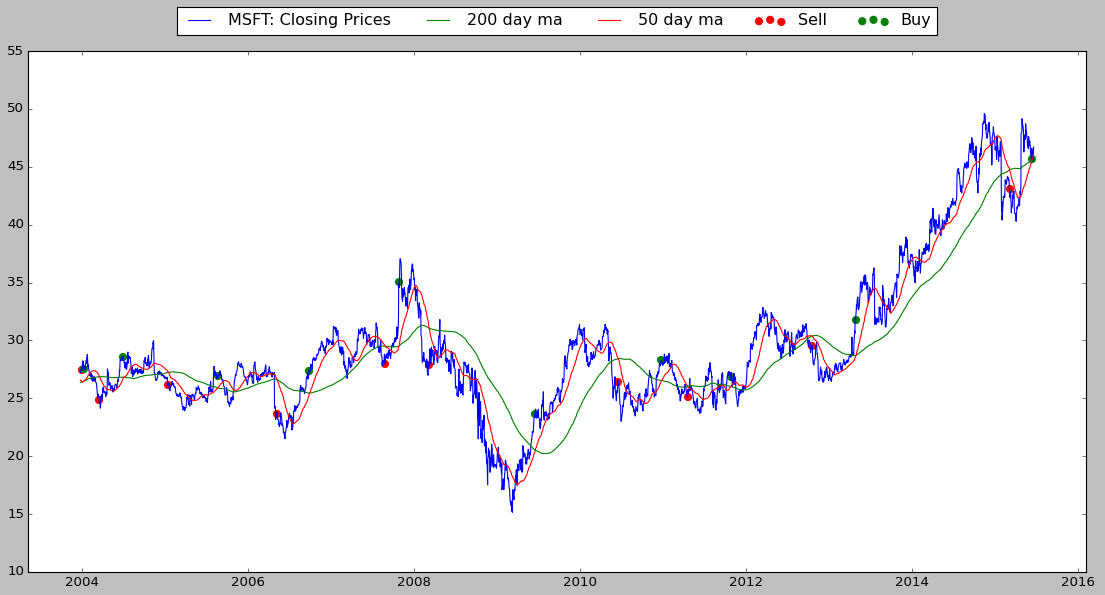
\includegraphics[width=\textwidth]{MSFT_BIG}
  \end{center}
      \caption{Moving Average MSFT}
\end{figure}

Die blaue Linie auf diesem Schaubild ist der Preis der Aktie. Die rote Kurve der Moving Average der letzten 50 Tage und die grüne Kurve der Moving Average der letzten 200 Tage. Immer wenn sich die Moving Average Kurven schneiden sieht man entweder einen grünen oder einen roten Punkt. Bei einem grünen Punkt soll die Aktie gekauft und bei einem roten verkauft werden.

\subsubsection{Ergebnisse}

Auch diesen Algorithmus wollten wir nicht nur an einzelnen Aktien testen da uns robuste Ergebnisse wichtig waren. In der ersten Spalte unserer Ergebnistabelle stehen die Aktienkurse mit denen der Algorithmus getestet wurde. Die Random Combinations bestehen aus 100 zufällig gewählten Aktienkursen. 

\begin{center}
\begin{tabularx}{\textwidth}{|X|X|}
\hline
Stock(s) used & Outcome\\
\hline
\hline
MSFT\footnote{Microsoft Corporation\texttrademark} & 13.39 \$\\
\hline
MCD\footnote{McDonald's Corp\texttrademark} & 2.71 \$\\
\hline
YHOO\footnote{Yahoo! Inc.\texttrademark} & 20.05 \$\\
\hline

NVDA\footnote{NVIDIA Corporation\texttrademark} & \textcolor{red}{-13.70 \$}\\
\hline
INTC\footnote{Intel Corporation\texttrademark} & 5.70 \$\\
\hline
AMZN\footnote{Amazon.com Inc.\texttrademark} & 128.87 \$\\
\hline
\hline
Random combination 1. & 34.53 \$\\
\hline
Random combination 2. &\textcolor{red}{-17.32 \$}\\
\hline
Random combination 3. & 56.94 \$\\
\hline
Random combination 4. & 15.74 \$\\
\hline
\end{tabularx}
\\[5pt]
Tabelle 2. Ergebnisse der Moving Average Algorithmus
\end{center}

In dieser Tabelle kann man sehen, dass wir durchaus gute Ergebnisse mit diesem Algorithmus erziehlt haben. Diese Tabelle beruht auf den Aktienkursen der letzten 1000 Tage. Wenn wir uns nur die Random Combinations anschauen, stellen wir fest das wir insgesamt 89.89\$ Gewinn gemacht haben. Jedoch ist dieses Positive Ergebnis keine Garantie dafür, das der selbe Test noch einmal so positiv ausfallen würde. Dennoch sind wir zufrieden mit unseren Testergebnissen. 


%----------------------------------------------------------------------------------------
%	MAJOR SECTION X - TEMPLATE - UNCOMMENT AND FILL IN
%----------------------------------------------------------------------------------------

%\section{Content Section}

%\subsection{Subsection 1} % Sub-section

% Content

%------------------------------------------------

%\subsection{Subsection 2} % Sub-section

% Content

%----------------------------------------------------------------------------------------
%	CONCLUSION
%----------------------------------------------------------------------------------------

\section{Fazit} % Major section

Das Fazit unserer Arbeit ist, dass es durchaus möglich ist mittels unserer Algorithmen
gute Ergebnisse zu erzielen. Dennoch ist uns das, trotz dem anpassen sämtlicher Parameter nicht mit allen Algorithmen gelungen. Das liegt vor allem daran, dass der Aktienmarkt sehr schnelllebig und teilweise unberechenbar ist. Die besten Ergebnisse hatten wir mit unserem Moving Average Algorithmus da dieser eher auf langfristige Vorhersagen ausgelegt ist und man somit auch leichte Fehlvorhersagen gut ausgleichen kann.

\section{Ausblick}

In der Zukunft könnte man unsere Algorithmen noch mit einem News-Crawler verbinden der verschiedene Nachrichtenseiten nach Neuigkeiten durchsucht.Diese Neuigkeiten könnten dann verwendet werden um eventuelle Veränderungen am Aktienmarkt besser und schneller vorherzusagen.


%----------------------------------------------------------------------------------------
%	BIBLIOGRAPHY
%----------------------------------------------------------------------------------------


%----------------------------------------------------------------------------------------

\end{document}